%   ------------------------------------------------------------------------
\FloatBarrier
\section{Análise do Pixie.haus}
\label{s.pixieHaus}

A plataforma Pixie.haus foi selecionada por seu grande potencial, sendo uma ferramenta com foco específico na geração de imagens e animações em pixel art. Uma de suas funcionalidades é o editor de imagens diretamente integrado na plataforma (Figura \ref{fig:pixieHausEditor}, o que, em tese, possibilitaria a correção rápida de pequenos erros e facilitaria o processo de ajuste fino dos resultados.

O objetivo principal do experimento é produzir a animação da porta B do cenário (apresentada anteriormente na Figura \ref{fig:portaB}) abrindo em uma perspectiva lateral.

Na geração de imagem, existem algumas opções de customização (Figura \ref{fig:pixieHausGeraImagem} no Apêndice \ref{ap.telasIA}) como a resolução, paleta de cores,  remoção do fundo e seleção do modelo de IA, sendo FLUX1.schnell e Luma Photon Flash os mais recomendados (Figura \ref{fig:pixieHausRecomenda} no Apêndice \ref{ap.telasIA}). Enquanto isso, na geração de vídeo é possível apenas adicionar uma imagem de referência e escolher o modelo de IA. 

Durante a preparação, foi encontrada uma limitação significativa da ferramenta: a funcionalidade de imagem de referência só aceita artes criadas na plataforma, sem opções para importar sprites externos. Isso exigiu que a porta fosse recriada manualmente. O editor, contudo, mostrou-se extremamente fraco, com ausência de ferramentas essenciais como seleção de área, exibição de coordenadas e precisão no preenchimento, tornando o processo pouco eficiente. Além disso, as funcionalidades existentes nesse editor só podiam ser utilizadas através de atalhos, descritos em uma interface separada. 

Foram disponibilizados créditos suficientes para a geração de duas animações, utilizando o modelo de texto e imagem para vídeo ByteDance Seedance-1-Lite. Em cada tentativa, foi usado um prompt diferente: o primeiro focando em especificar a ação de maneira direta e com precisão (Figura \ref{fig:pixieHausPrompt1}), e o segundo com uma descrição mais técnica sobre como os frames deveriam se comportar (Figura \ref{fig:pixieHausPrompt2}).

\begin{figure}[htbp]
    \centering
    \caption{\small Primeiro prompt utilizado no Pixie.Haus}
    \label{fig:pixieHausPrompt1}
    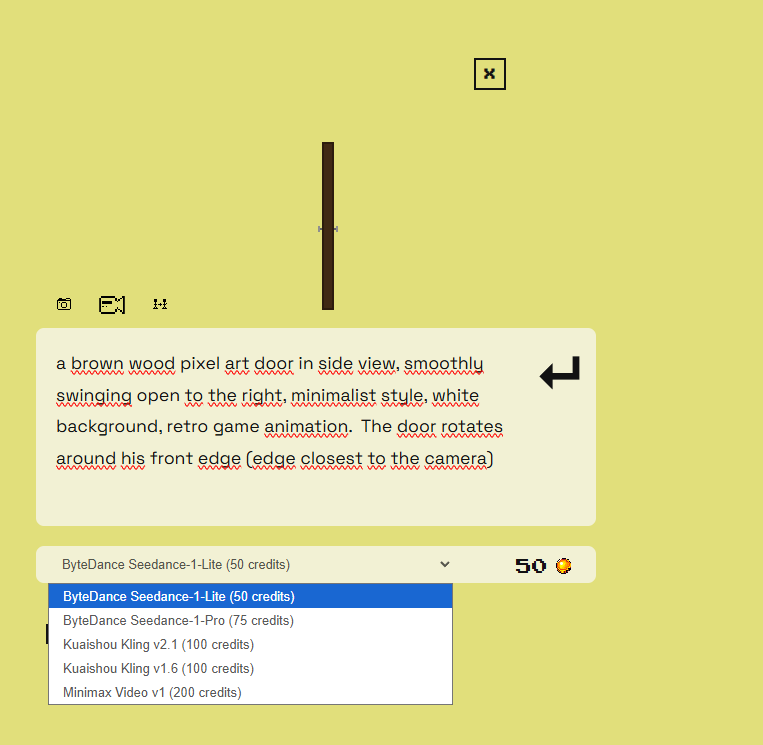
\includegraphics[width=0.6\linewidth]{figs/pixieHaus/tela2.PNG}
    \legend{\small Fonte: Elaborada pela autora.}
\end{figure}

\begin{figure}[htbp]
    \centering
    \caption{\small Segundo prompt utilizado no Pixie.Haus}
    \label{fig:pixieHausPrompt2}
    \begin{subfigure}{0.45\linewidth}
        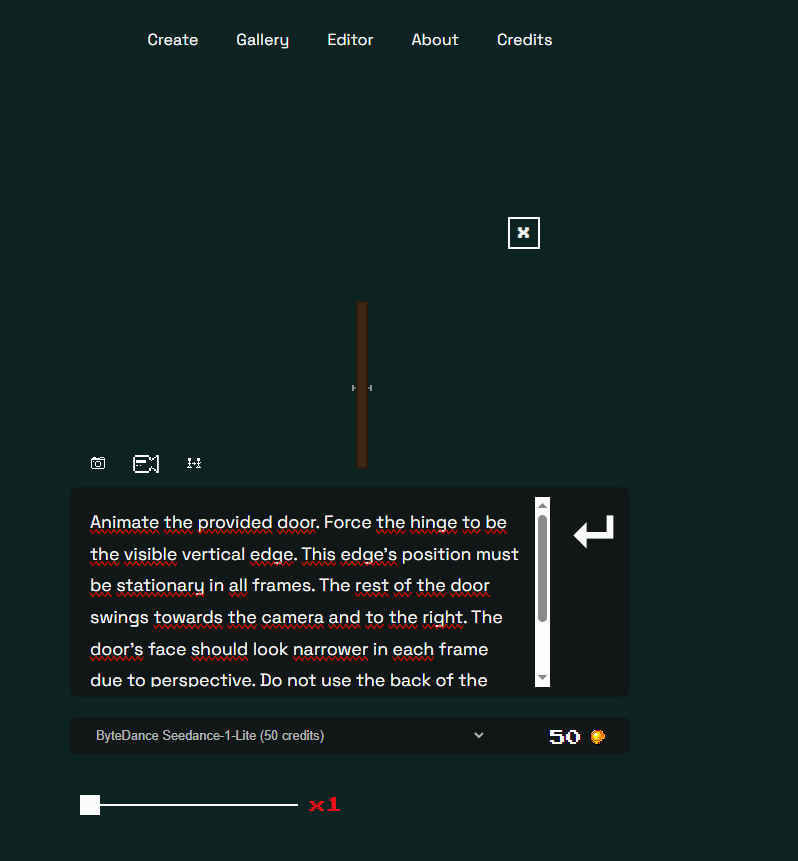
\includegraphics[width=1\linewidth]{figs/pixieHaus/tela3.PNG}
        \caption{\small Primeira parte do prompt}
        \label{fig:pixieHausPrompt2a}
    \end{subfigure}
    \begin{subfigure}{0.45\linewidth}
        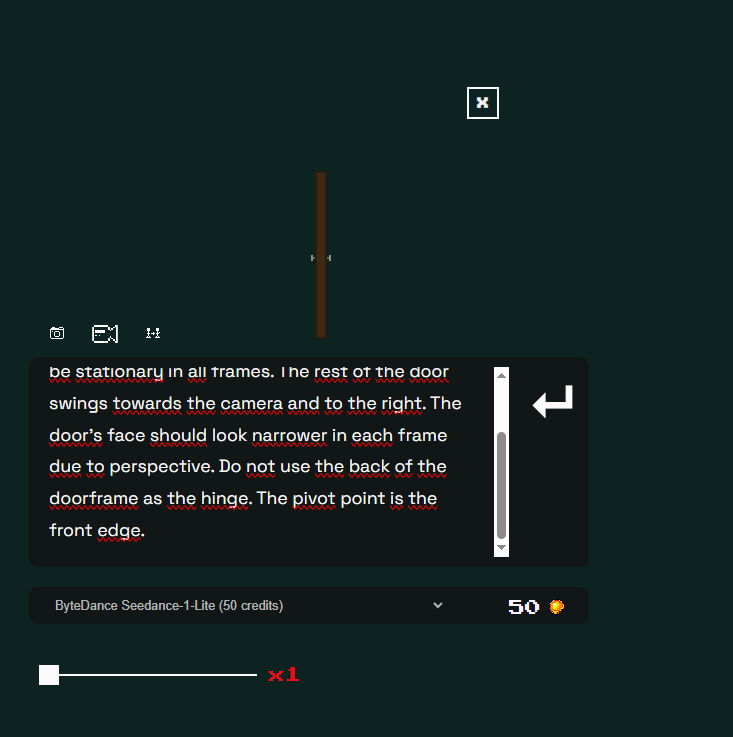
\includegraphics[width=1\linewidth]{figs/pixieHaus/tela4.PNG}
        \caption{\small Segunda parte do prompt}
        \label{fig:pixieHausPrompt2b}
    \end{subfigure}
    \legend{\small Fonte: Elaborada pela autora.}
\end{figure}

Ambas as tentativas produziram resultados insatisfatórios\footnote{https://drive.google.com/drive/folders/1rnU-I261vEqKgXC7RwA23u1XItUGiDwM?usp=sharing}. O principal problema foi a falha da ferramenta em gerar o movimento de abertura solicitado. No primeiro teste, a IA criou uma animação onde a porta se materializa deslizando horizontalmente antes de abrir incorretamente em front view. No segundo, além da porta se materializar da mesma forma que ocorreu no resultado anterior, foi feita uma rotação completa da porta sobre seu eixo central. A IA aparenta ter interpretado o prompt inicial como sendo apenas uma parte incompleta da porta. As Figuras \ref{fig:pixieHaus1} e \ref{fig:pixieHaus2} apresentam frames de ambas as animações geradas.

\begin{figure}[htbp]
    \centering
    \caption{\small Frames da animação gerada pelo prompt 1}
    \label{fig:pixieHaus1}
    \begin{subfigure}{0.45\linewidth}
        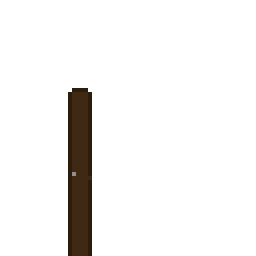
\includegraphics[width=1\linewidth]{figs/pixieHaus/2frame1.PNG}
        \caption{\small Frame da animação}
        \label{fig:pixieHaus1a}
    \end{subfigure}
    \begin{subfigure}{0.45\linewidth}
        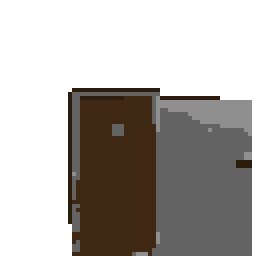
\includegraphics[width=1\linewidth]{figs/pixieHaus/2frame2.PNG}
        \caption{\small Frame posterior da animação}
        \label{fig:pixieHaus1b}
    \end{subfigure}
    \legend{\small Fonte: Elaborada pela autora, utilizando a ferramenta Pixie.Haus.}
\end{figure}

\begin{figure}[htbp]
    \centering
    \caption{\small Frames da animação gerada pelo prompt 2}
    \label{fig:pixieHaus2}
    \begin{subfigure}{0.45\linewidth}
        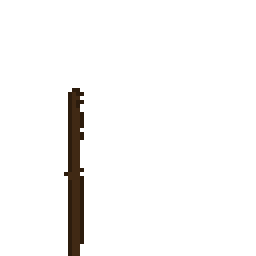
\includegraphics[width=1\linewidth]{figs/pixieHaus/1frame1.PNG}
        \caption{\small Frame da animação}
        \label{fig:pixieHaus2a}
    \end{subfigure}
    \begin{subfigure}{0.45\linewidth}
        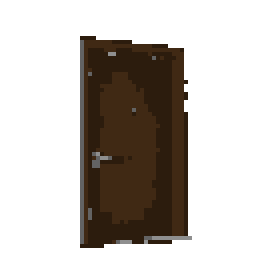
\includegraphics[width=1\linewidth]{figs/pixieHaus/1frame2.PNG}
        \caption{\small Frame posterior da animação}
        \label{fig:pixieHaus2b}
    \end{subfigure}
    \legend{\small Fonte: Elaborada pela autora, utilizando a ferramenta Pixie.Haus.}
\end{figure}

Adicionalmente, foi observada uma falha no pós-processamento de remoção de fundo\footnote{Além da animação final, a ferramenta também disponibilizou automaticamente o estado do vídeo antes do fundo ser removido}, que manteve a sombra da porta e a deformação do fundo como parte do sprite, o que pode ser verificado na Figura \ref{fig:pixieHausSombra}. Embora os resultados mantivessem o estilo correto e um padrão pixel perfect, a imprecisão na interpretação das instruções textuais foi o problema mais crítico.

\begin{figure}[htbp]
    \centering
    \caption{\small Inclusão incorreta da sombra}
    \label{fig:pixieHausSombra}
    \begin{subfigure}{0.45\linewidth}
        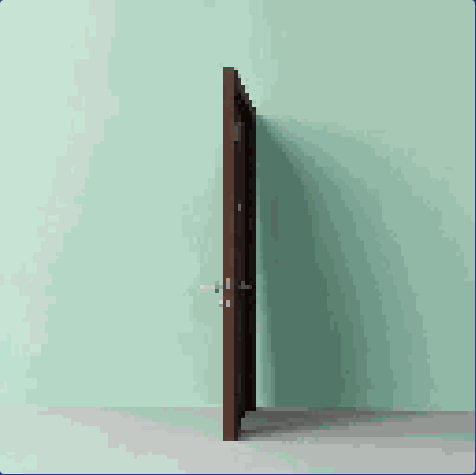
\includegraphics[width=1\linewidth]{figs/pixieHaus/1sombraFundo.PNG}
        \caption{\small Frame da animação com fundo}
        \label{fig:pixieHausSombra1a}
    \end{subfigure}
    \begin{subfigure}{0.35\linewidth}
        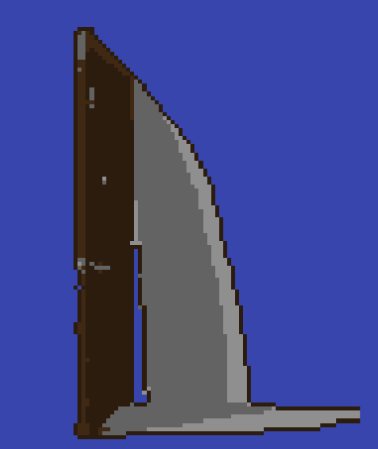
\includegraphics[width=1\linewidth]{figs/pixieHaus/1sombra.PNG}
        \caption{\small Frame da animação após a remoção de fundo}
        \label{fig:pixieHausSombra1b}
    \end{subfigure}
    \legend{\small Fonte: Elaborada pela autora, utilizando a ferramenta Pixie.Haus.}
\end{figure}


Como a análise da Pixie.haus foi restringida pelo seu limitado modelo de créditos gratuitos, não foi possível testar outros modelos e prompts. Com base nos poucos testes realizados, a ferramenta foi descartada, pois as animações geradas se mostraram imprecisas e inadequadas para o objetivo do projeto. Apesar disso, a plataforma apresenta um conceito promissor com falhas na execução. Embora a integração de um editor de pixel art tenha como objetivo a praticidade, sua implementação atual não é adequada para edições complexas e não permite editar os GIFs finais gerados.

No entanto, o principal diferencial da ferramenta é sua capacidade de gerar resultados pixel perfect. Este padrão é alcançado através de uma série de etapas de pós-processamento, que incluem o redimensionamento pelo método do nearest neighbor (vizinho mais próximo, em inglês) para manter as bordas mais nítidas, o ajuste da paleta de cores para garantir consistência e a remoção de fundo. Essa característica assegura que os sprites gerados possam ser facilmente manipulados em softwares de edição externos de pixel art sem sofrer distorção. Isso confere à Pixie.haus um grande potencial que, no momento, não pôde ser plenamente explorado. % devido à baixa performance do seu modelo de IA na interpretação de prompts de animação.

%devido aos créditos limitados, na real
